% -------------------------------------------------------------------------------------- %

\section{Numerical Example: Landau Damping}\label{sec:landau}

\begin{figure}
    \centering
    \begin{subfigure}{0.45\textwidth}
        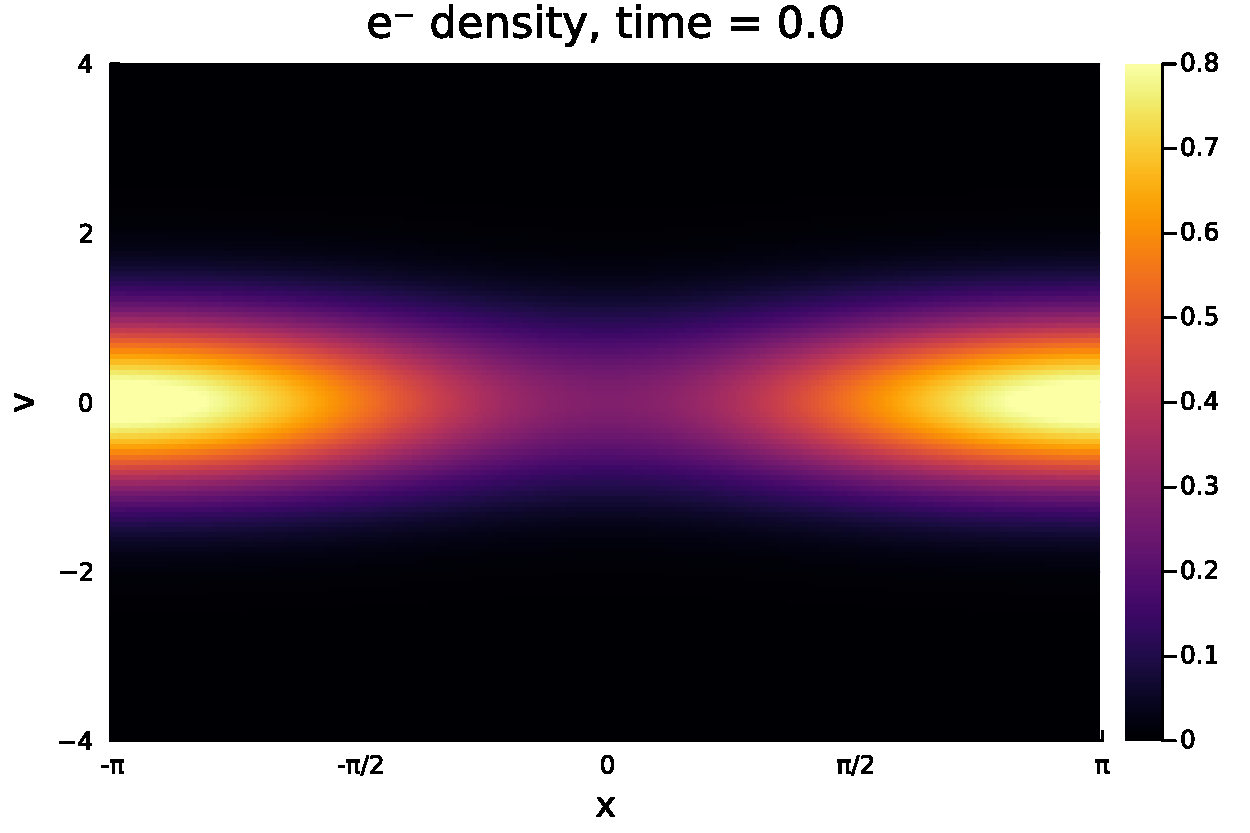
\includegraphics[width=\textwidth]{e_density_t0.pdf}
    \end{subfigure}
    \begin{subfigure}{0.45\textwidth}
        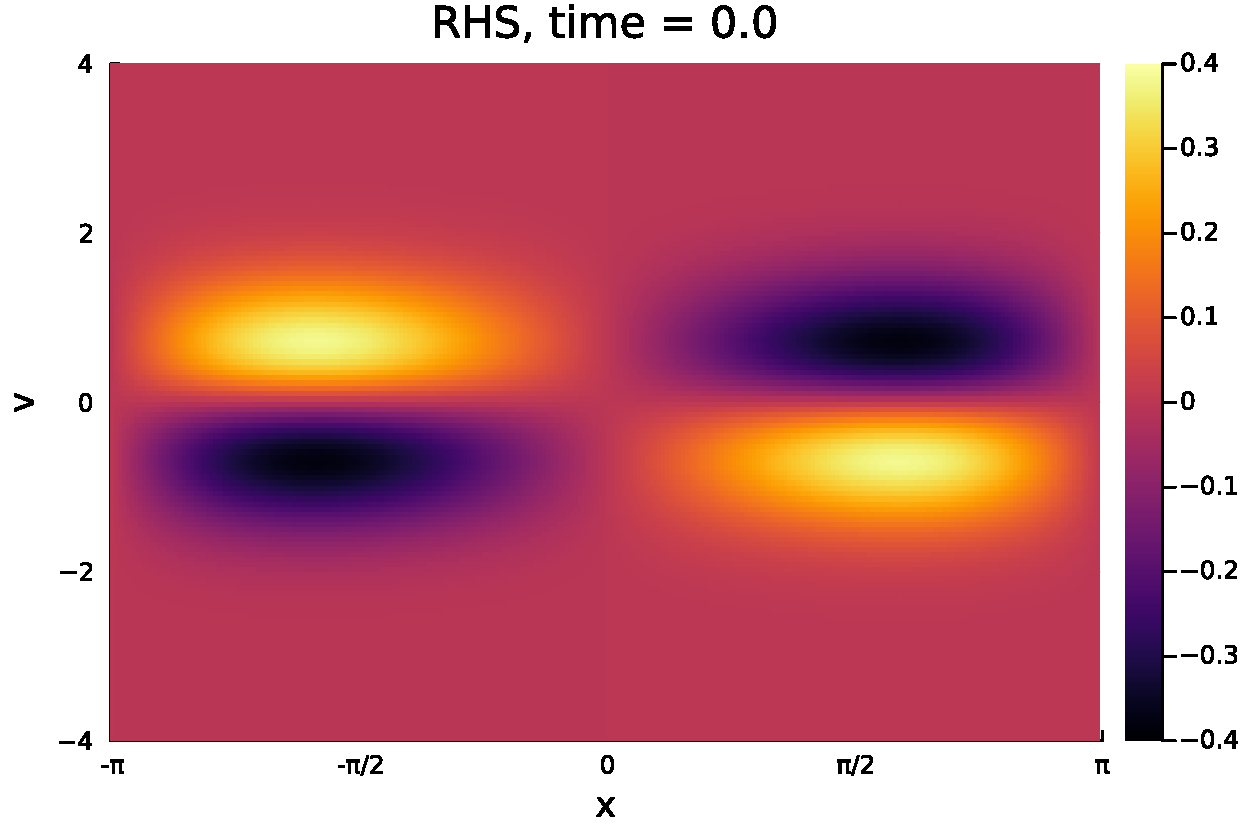
\includegraphics[width=\textwidth]{rhs_t0.pdf}
    \end{subfigure}
    \begin{subfigure}{0.45\textwidth}
        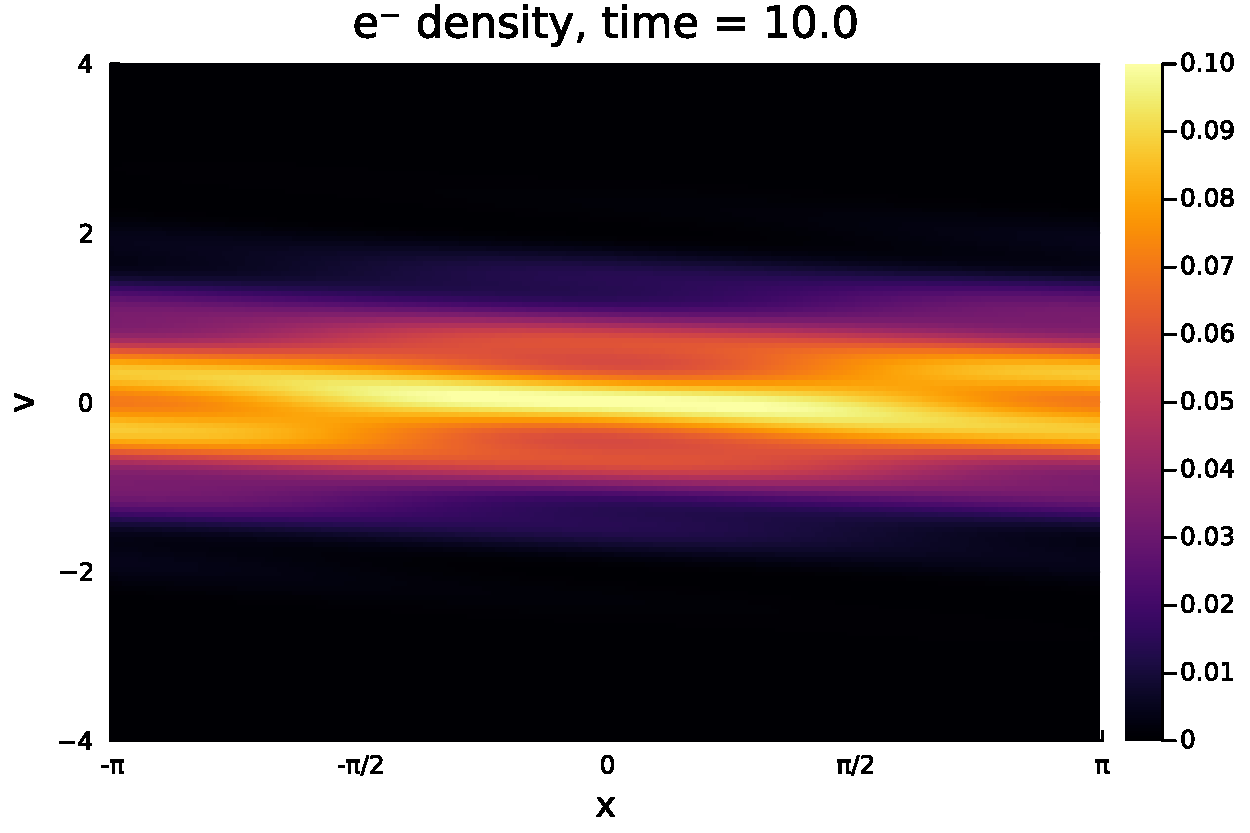
\includegraphics[width=\textwidth]{e_density_t10.pdf}
    \end{subfigure}
    \begin{subfigure}{0.45\textwidth}
        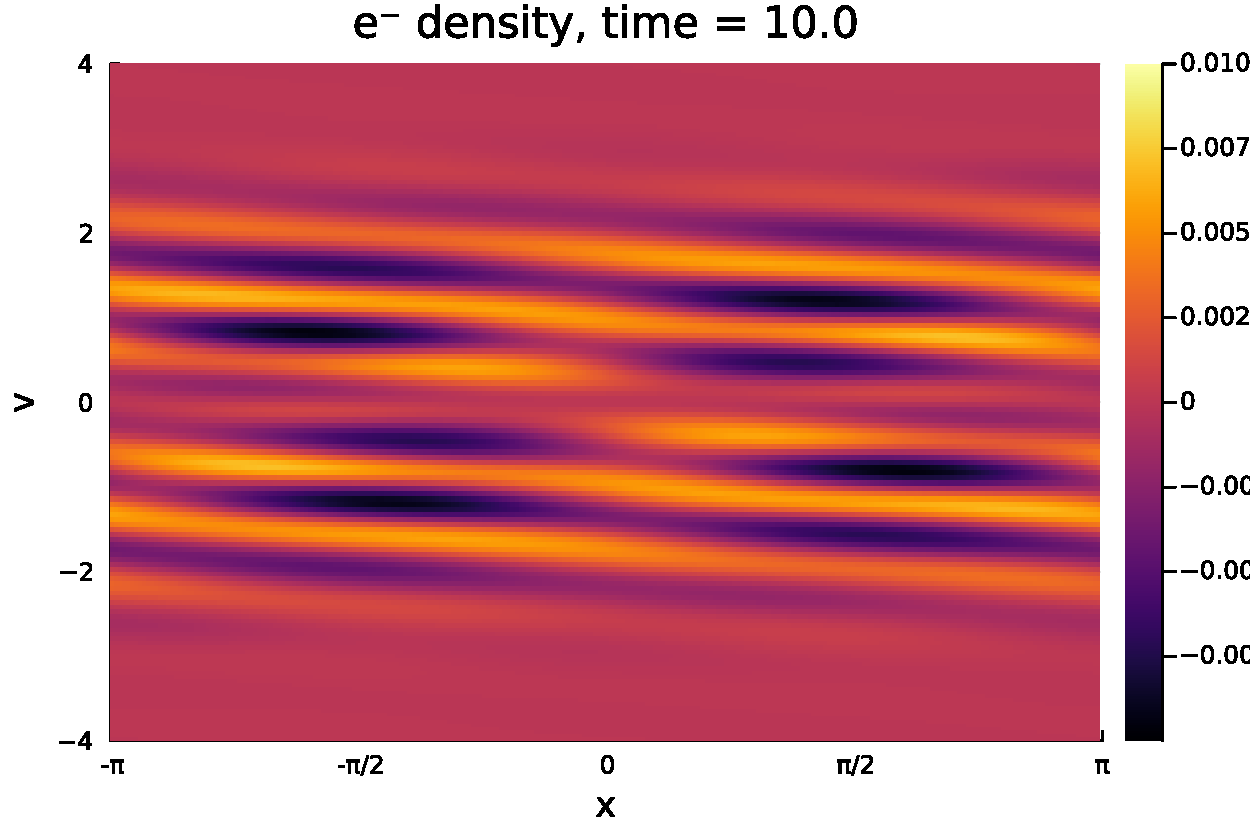
\includegraphics[width=\textwidth]{rhs_t10.pdf}
    \end{subfigure}
    \caption{
        Landau damping. Density \ref{eq:initial_conditions} and RHS for various times. 
        !! Note the differing color bar axes!
    }\label{fig:density}
\end{figure}

\begin{figure}
    \centering
    \begin{subfigure}{0.45\textwidth}
        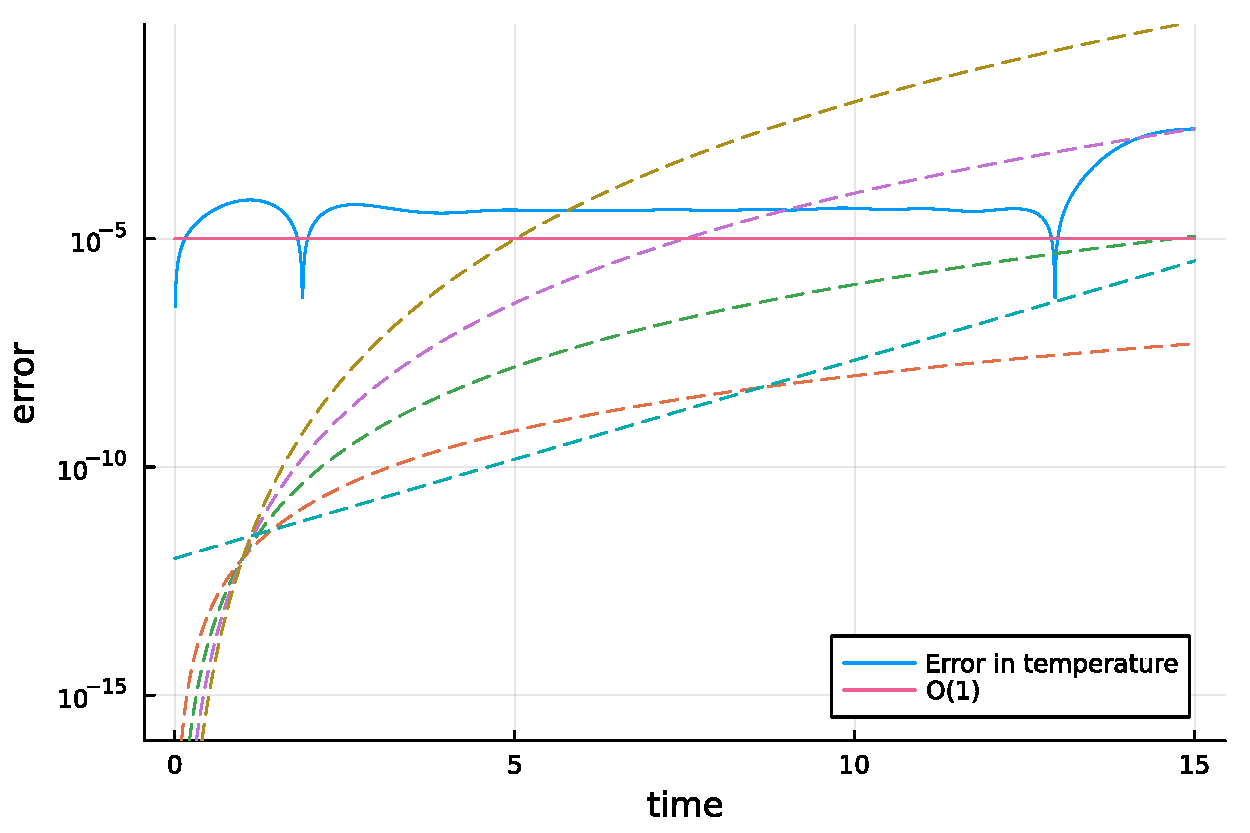
\includegraphics[width=\textwidth]{2th_moment_error.pdf}
    \end{subfigure}
    \begin{subfigure}{0.45\textwidth}
        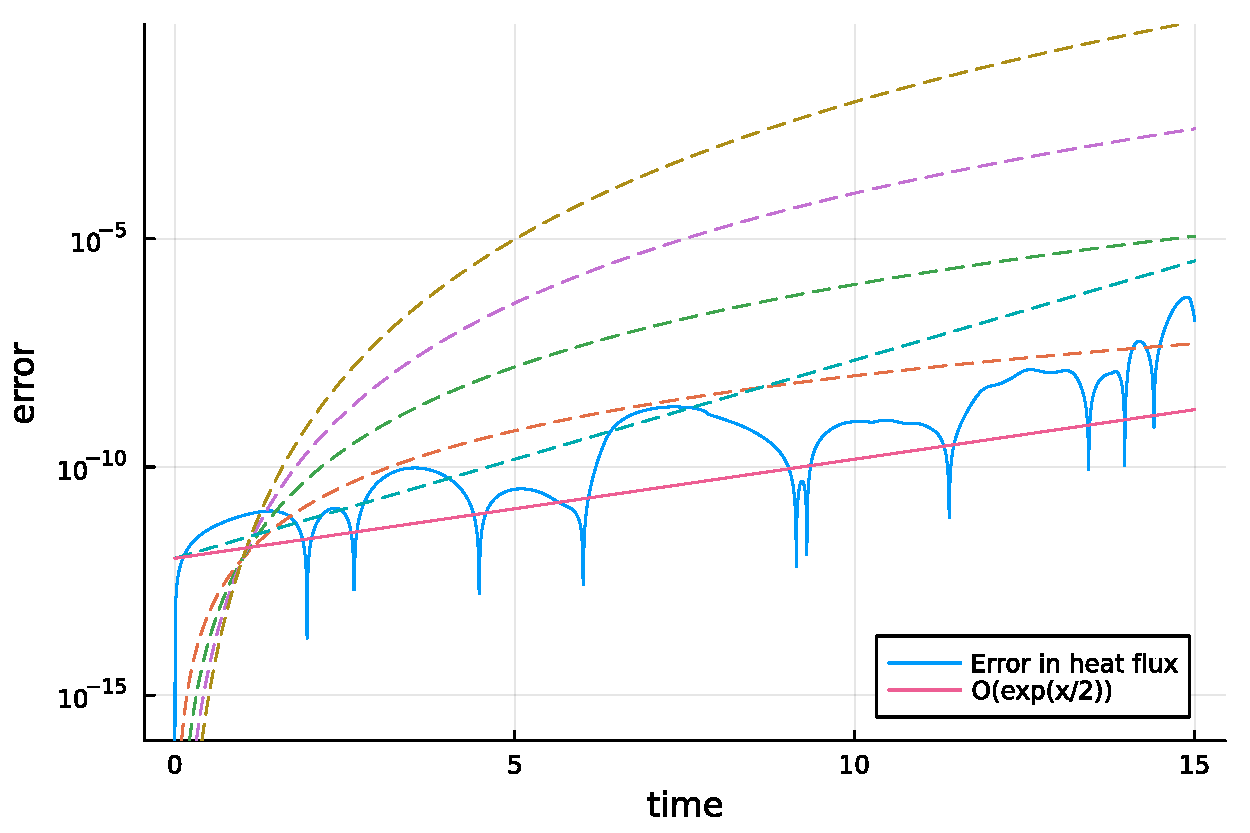
\includegraphics[width=\textwidth]{3th_moment_error.pdf}
    \end{subfigure}
    \begin{subfigure}{0.45\textwidth}
        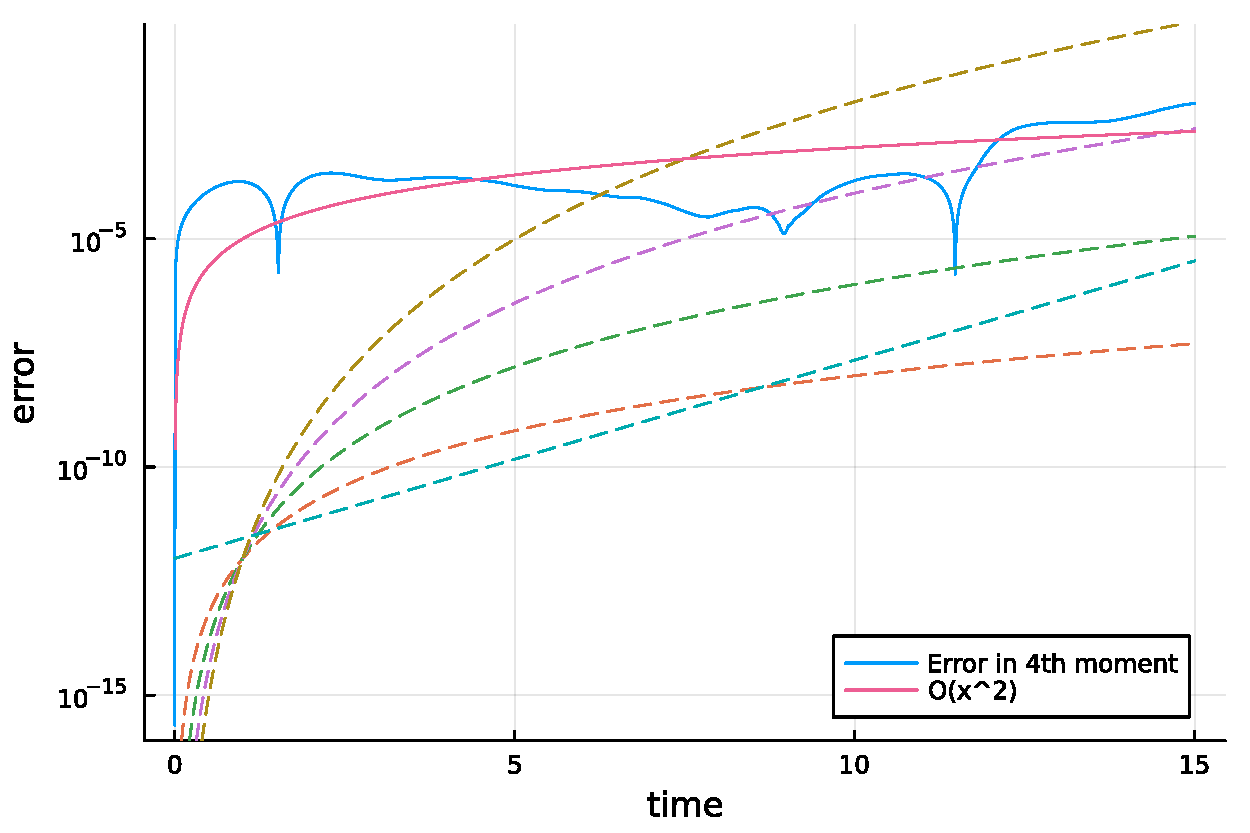
\includegraphics[width=\textwidth]{4th_moment_error.pdf}
    \end{subfigure}
    \begin{subfigure}{0.45\textwidth}
        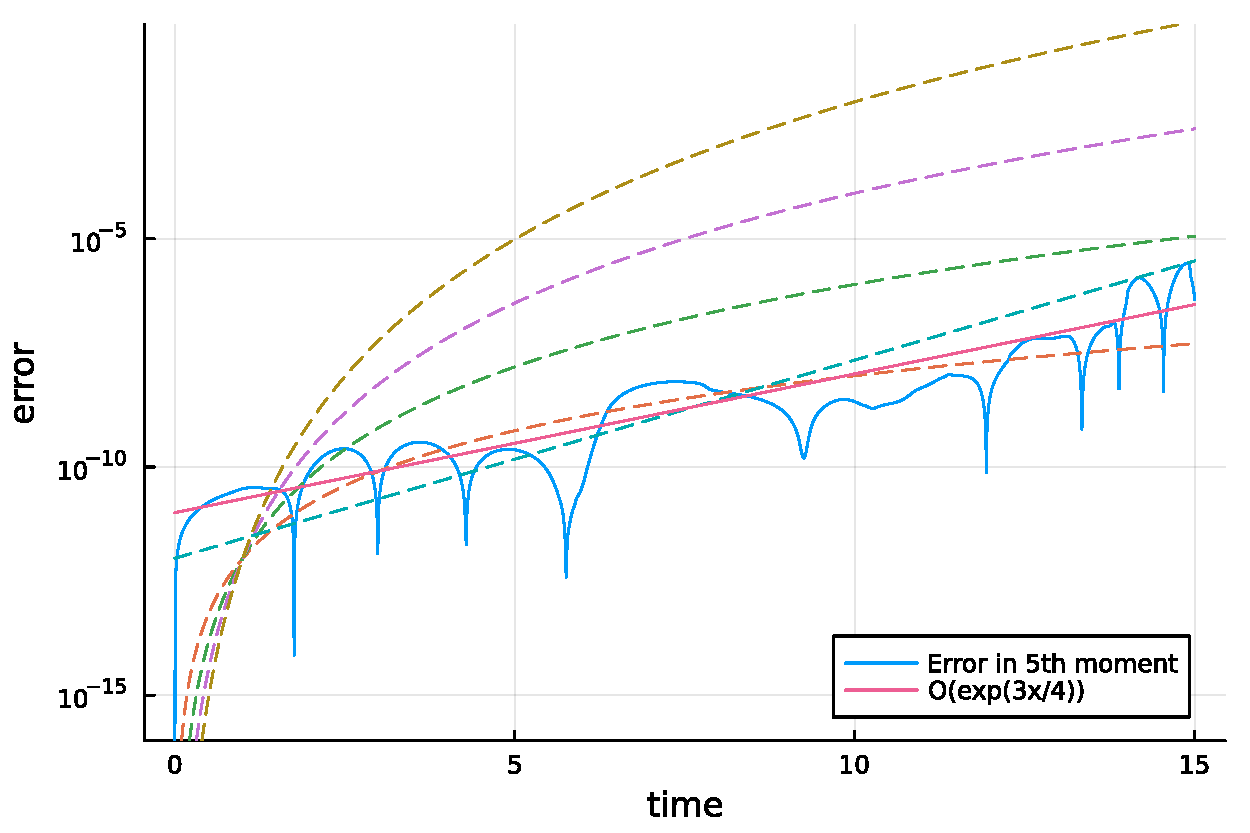
\includegraphics[width=\textwidth]{5th_moment_error.pdf}
    \end{subfigure}
    \begin{subfigure}{0.45\textwidth}
        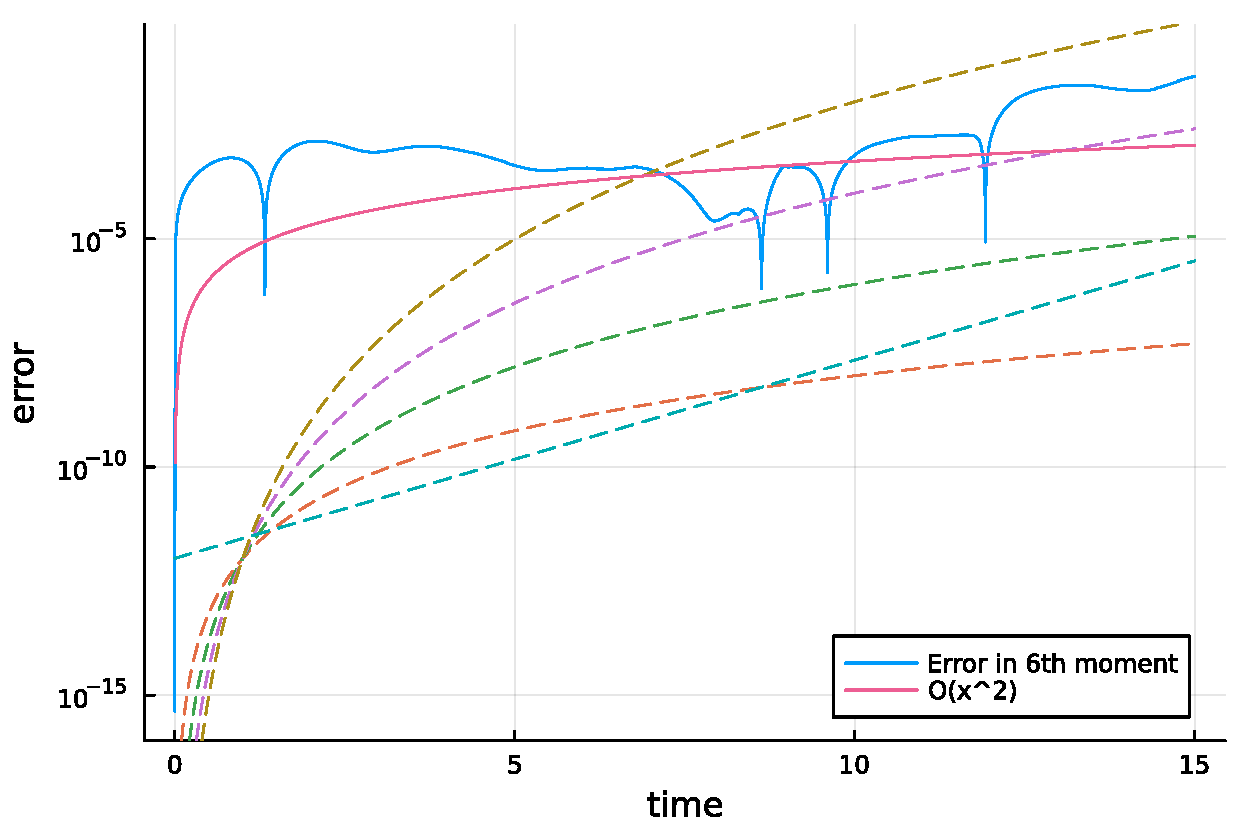
\includegraphics[width=\textwidth]{6th_moment_error.pdf}
    \end{subfigure}
    \begin{subfigure}{0.45\textwidth}
        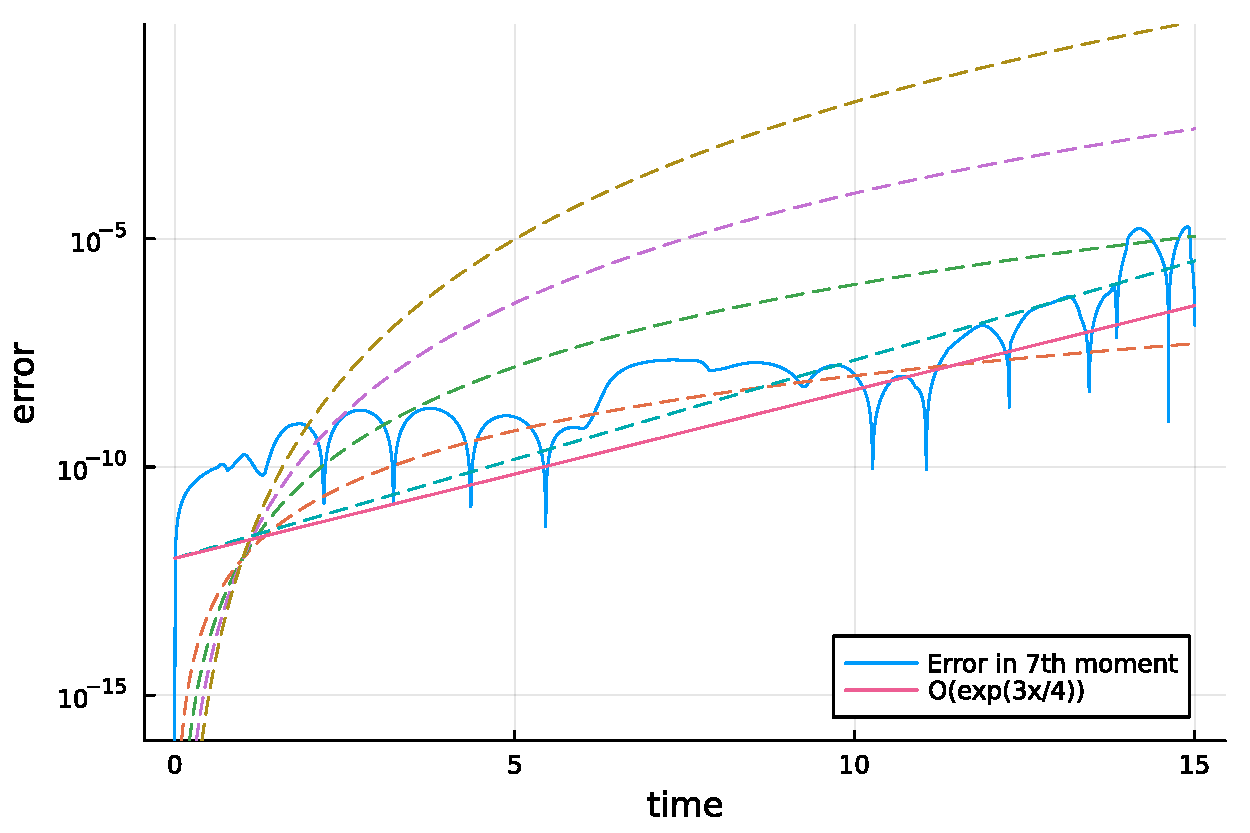
\includegraphics[width=\textwidth]{7th_moment_error.pdf}
    \end{subfigure}
    \caption{
        Even- and odd-power moment errors based on one very exact numerical integration. 
        Dashed overlay are various power laws: orange: $O(\tau^4)$, green: $O(\tau^6)$, pink: 
        $O(\tau^4)$, yellow: $O(\tau^10)$, light blue: $O(exp(\tau))$. 
    }\label{fig:moments}
\end{figure}

\iffalse
\begin{figure}
    \missingfigure{}
    \caption{
        Conservation of observables until $f$ becomes negative
    }\label{fig:positivity}
\end{figure}
\fi

\begin{enumerate}
    \item Basic takeaway of Landau damping: dissipation can occur without loss of energy; 
          different than in fluid equations
    \item Specific initial conditions that we consider: 
          \begin{equation}\label{eq:initial_conditions}
            f (x, v, 0) = ( 1 + \alpha \cos (x) ) \exp (- v^2)
          \end{equation}
          for the parameter value $\alpha = 1/2$ computed over the domain 
          $\Omega_x = [ -\pi, \pi )_{per}$, $\Omega_v = [ -5, 5 ]$. $f$ is normalized 
          to have initial mass $1$. 
    \item This is too large of a parameter value to use linear approx from Landau's 
          original argument, but the derivation can be done to higher order and 
          dissipation is still analytically predicted. Indeed, we see this numerically as 
          well, see fig. \ref{fig:density}. 
    \item Odd power moments seem to have very predictable behavior. The error follows a 
          power/exponential law very well (see fig. \ref{fig:moments}). This must have something to 
          do with some form of symmetry wrt. $\Omega_v$. Are the kinetic moment density 
          functions 
          \begin{equation}
            \underbrace{v v \ldots v}_{k\text{ times}} f(x, v, t)
          \end{equation}
          symmetric wrt. $v$? All odd moments $\scrM_k$ are essentially $0$. Even power 
          moments seem more erratic but are lower long-term. This could be a power law, 
          though it is difficult to tell. Another, longer integration may be needed. 
    \item Observables seem to be near-constant whenever the density function is 
          positive, see fig. \ref{fig:positivity}. As soon as $f$ becomes negative, the 
          observables go haywire. Should a positivity-preserving method be considered? 
          How would this affect the conservation? 
\end{enumerate}

% -------------------------------------------------------------------------------------- %
